\documentclass[conference]{IEEEtran}
\IEEEoverridecommandlockouts
\usepackage{cite}
\usepackage{amsmath,amssymb,amsfonts}
\usepackage{graphicx}
\usepackage{textcomp}
\usepackage{xcolor}
\usepackage{array}
\usepackage{booktabs}
\usepackage{tikz}
\usetikzlibrary{shapes.geometric, arrows.meta, positioning, fit, backgrounds}

% TikZ styles for architecture diagram
\tikzstyle{block} = [rectangle, rounded corners=3pt,
  minimum width=3.2cm, minimum height=0.7cm,
  text centered, draw=black, fill=blue!8, font=\small]
\tikzstyle{decision} = [diamond, minimum width=2cm,
  minimum height=0.6cm, text centered, draw=black,
  fill=orange!15, font=\scriptsize]
\tikzstyle{arrow} = [thick,->,>=stealth]
\tikzstyle{thread1} = [rectangle, rounded corners=3pt,
  minimum width=3.4cm, minimum height=0.7cm,
  text centered, draw=black, fill=green!10, font=\small]
\tikzstyle{thread2} = [rectangle, rounded corners=3pt,
  minimum width=3.4cm, minimum height=0.7cm,
  text centered, draw=black, fill=purple!10, font=\small]
\tikzstyle{output} = [rectangle, rounded corners=3pt,
  minimum width=3.2cm, minimum height=0.7cm,
  text centered, draw=black, fill=yellow!10, font=\small]

\begin{document}

% ── TITLE ───────────────────────────────────────────────────
\title{Real-Time Facial Emotion Recognition System to Support
Autistic Children During Classroom Learning}

\author{
  \IEEEauthorblockN{Darshan G K}
  \IEEEauthorblockA{
    \textit{PG Scholar, ASAC}\\
    \textit{Alliance University, Bangalore}\\
    gdarshanMTECH25@stu.alliance.edu.in
  }
  \and
  \IEEEauthorblockN{Shreenidhi H S}
  \IEEEauthorblockA{
    \textit{Professor, ASAC}\\
    \textit{Alliance University, Bangalore}\\
    shreenidhi.hs@alliance.edu.in
  }
}

\maketitle

% ── ABSTRACT ────────────────────────────────────────────────
\begin{abstract}
Autism Spectrum Disorder (ASD) is a neurodevelopmental condition
affecting approximately 1 in 100 children worldwide, with India
recording around 1 in 68 school-going children on the spectrum.
One of the most pressing challenges in Indian special schools is
that teachers have no affordable, real-time tool to monitor the
emotional state of an autistic child during a classroom session.
Children with ASD often struggle to verbally express emotions
such as frustration, confusion, anxiety, or happiness, creating
a communication gap that hampers their learning and well-being.
This paper presents a prototype real-time facial emotion
recognition system, EmoSense AI, designed to run on a standard
laptop webcam with no additional hardware or internet access.
The system uses OpenCV for frame capture and DeepFace for
emotion classification into a small set of categories derived
from the available model output. A simple Flask dashboard
provides live session status, confidence information, and
offline alert handling via pyttsx3. The implementation is a
practical classroom prototype rather than a fully validated
clinical system. The project is evaluated on a small
experimental subset of ASD-related image data where available,
and results are reported as preliminary evidence demonstrating
that general-purpose FER models can be sensitive to ASD-specific
facial variation. Future work should focus on data collection,
model tuning, and field validation in real classrooms.
\end{abstract}

\begin{IEEEkeywords}
Autism Spectrum Disorder, Facial Emotion Recognition, Deep
Learning, Computer Vision, DeepFace, OpenCV, Assistive
Technology, Special Education, FER-Autism, Real-Time Detection,
Convolutional Neural Network, Flask, Teacher Dashboard
\end{IEEEkeywords}

% ── I. INTRODUCTION ─────────────────────────────────────────
\section{Introduction}

Autism Spectrum Disorder (ASD) is a complex neurodevelopmental
condition that affects social communication, behavior, and
emotional expression. The World Health Organization estimates
that approximately 1 in 100 children worldwide are diagnosed
with ASD, with India recording around 1 in 68 school-going
children on the spectrum~\cite{who2023}. One of the most
critical challenges in special education is that teachers in
inclusive and special schools have no affordable, real-time
tool to monitor the emotional state of an autistic child during
a classroom session.

Children with ASD often exhibit atypical facial expressions
that differ from neurotypical individuals in intensity, timing,
and specificity~\cite{trevisan2018}. This characteristic makes
it difficult for teachers to accurately interpret the child's
emotional state without specialized training or assistive
tools~\cite{leo2015}. The communication gap results in delayed
intervention, misunderstanding, and inappropriate support at
critical moments during learning.

The field of facial emotion recognition (FER) has advanced
significantly with deep learning. Goodfellow et al.
introduced the FER2013 dataset and showed that Convolutional
Neural Networks can automatically learn spatial features from
facial images~\cite{goodfellow2013}. However, models trained
on adult facial data consistently underperform when applied
to ASD children's expressions due to fundamental differences
in expressiveness patterns~\cite{radocaj2025,leo2015}.

Existing solutions for emotion monitoring in ASD children
require expensive hardware such as EEG headsets or IoT
sensors~\cite{talaat2023}, or internet connectivity
unavailable in most Indian special schools. No existing system
provides a teacher-facing real-time dashboard for ASD
classroom monitoring that operates on a standard laptop alone.

This report presents EmoSense AI as a prototype for local
emotion monitoring in classroom settings. The system combines
three core elements: (1) webcam-based face capture and emotion
inference through OpenCV and DeepFace; (2) a simple Flask web
interface for live status and recent history; and (3) optional
offline audio alerts for sustained negative expressions. The
implementation is intended for experimentation and iteration,
not as a final validated clinical or deployment-ready product.

% ── II. LITERATURE REVIEW ───────────────────────────────────
\section{Literature Review}

\subsection{Facial Emotion Recognition and Deep Learning}

The foundation of modern FER lies in large-scale annotated
datasets and deep learning architectures. Goodfellow et
al.~\cite{goodfellow2013} introduced the FER2013 dataset
and demonstrated that CNNs could achieve over 70\% accuracy
on real-world facial expression recognition without manual
feature engineering. This established CNNs as the dominant
approach for FER.

Serengil and Ozpinar~\cite{serengil2020} developed DeepFace,
an open-source framework that consolidates multiple pre-trained
face analysis models. DeepFace enables real-time emotion
inference using pre-trained CNNs without requiring custom
model training, making it accessible for applied research
systems such as EmoSense AI.

\subsection{Deep Learning for Emotion Recognition in ASD}

Rada\v{c}aj and Martinovi\'{c}~\cite{radocaj2025} conducted
a comprehensive study using ResNet, EfficientNet, and Vision
Transformers for emotion recognition in autistic children.
Their findings showed transformer-based models outperform
CNN architectures in detecting subtle ASD facial expressions.

Hosney et al.~\cite{hosney2024} proposed AuYOLO-Att, an
attention-based YOLOv8 model for early autism diagnosis
through facial expression recognition, advocating for
domain-adapted architectures rather than general-purpose
FER models trained on adult datasets.

Trevisan et al.~\cite{trevisan2018} conducted a meta-analysis
confirming that individuals with ASD demonstrate systematically
different facial expression patterns with significant
differences in expression intensity. This neurological basis
directly explains why general-purpose FER models underperform
on ASD data.

\subsection{Real-Time Assistive Systems}

Talaat~\cite{talaat2023} developed a real-time FER system
for autistic children combining deep learning with IoT
feedback. Published in \textit{Neural Computing and
Applications} (Springer), the study confirmed AI-based
emotion monitoring feasibility but required IoT hardware
unavailable in Indian schools.

Talaat~\cite{talaat2025} applied MobileNetV2 with
meta-learning to classify emotions from the Autistic Children
Emotions dataset, achieving 86\% testing accuracy.
This demonstrated that transfer learning can substantially
improve performance on domain-specific ASD datasets.

An IEEE-published study~\cite{ieee2024} presented an ASD
emotion detection system using OpenCV and Haar Cascade for
real-time face detection combined with a deep learning
classifier, confirming open-source tools are sufficient
for functional real-time assistive prototypes.

Jaffar and Abdulbaqi~\cite{jaffar2023} proposed a deep
learning framework for facial expression recognition of ASD
children, reinforcing that vision-based automatic recognition
is both technically feasible and practically needed in
educational settings.

\subsection{Datasets and Systematic Evidence}

A systematic review~\cite{systematic2024} covering 65
peer-reviewed studies found that video cameras and facial
expression analysis were the most widely used modality for
autism emotion recognition. The review identified a critical
gap: very few studies have been validated in real-world
classroom environments, particularly in developing countries.

The FER-Autism dataset~\cite{ferautism2025}, developed under
medical supervision at Kafrelsheikh University, Egypt,
contains 1,420 facial images of ASD children specifically
curated for emotion recognition research. It represents a
significant improvement over general-purpose adult datasets
such as FER2013 (2013) for ASD-specific evaluation and is
the primary evaluation dataset of this work.

Keating and Cook~\cite{keating2020} reviewed facial
expression production and recognition in ASD, noting that
shifting paradigms in research increasingly support
computer-vision approaches for automated emotion analysis
in clinical and educational settings.

\subsection{Indian Context and Government Alignment}

The Department of Empowerment of Persons with Disabilities
(DEPwD, 2024)~\cite{depwd2024} has documented ten active
SIPDA-funded research projects targeting disability
technology for children, confirming that AI-powered
assistive tools for special children are a national
research priority. None of the funded projects deploy
a real-time CV-based emotion monitoring system for
classroom use, confirming a significant unmet need.

\subsection{Research Gap}

Three critical gaps remain unaddressed: (1) no validated
real-time FER system has been deployed in an Indian special
school classroom context; (2) existing systems do not provide
a teacher-facing dashboard with session history, audio alerts,
and session export for non-technical educators; and
(3) all reviewed systems require internet, IoT hardware, or
specialized devices --- none are deployable on a standard
laptop alone. EmoSense AI directly addresses all three gaps.

% ── III. PROPOSED METHODOLOGY ───────────────────────────────
\section{Proposed Methodology}

\subsection{System Architecture}

The EmoSense AI system consists of three integrated modules
running locally on a standard laptop: (1) Face Detection and
Emotion Classification, (2) Teacher Dashboard, and
(3) Audio Alert System. Fig.~\ref{fig:arch} shows the
complete system architecture.

% ── ARCHITECTURE DIAGRAM ────────────────────────────────────
\begin{figure}[h]
\centering
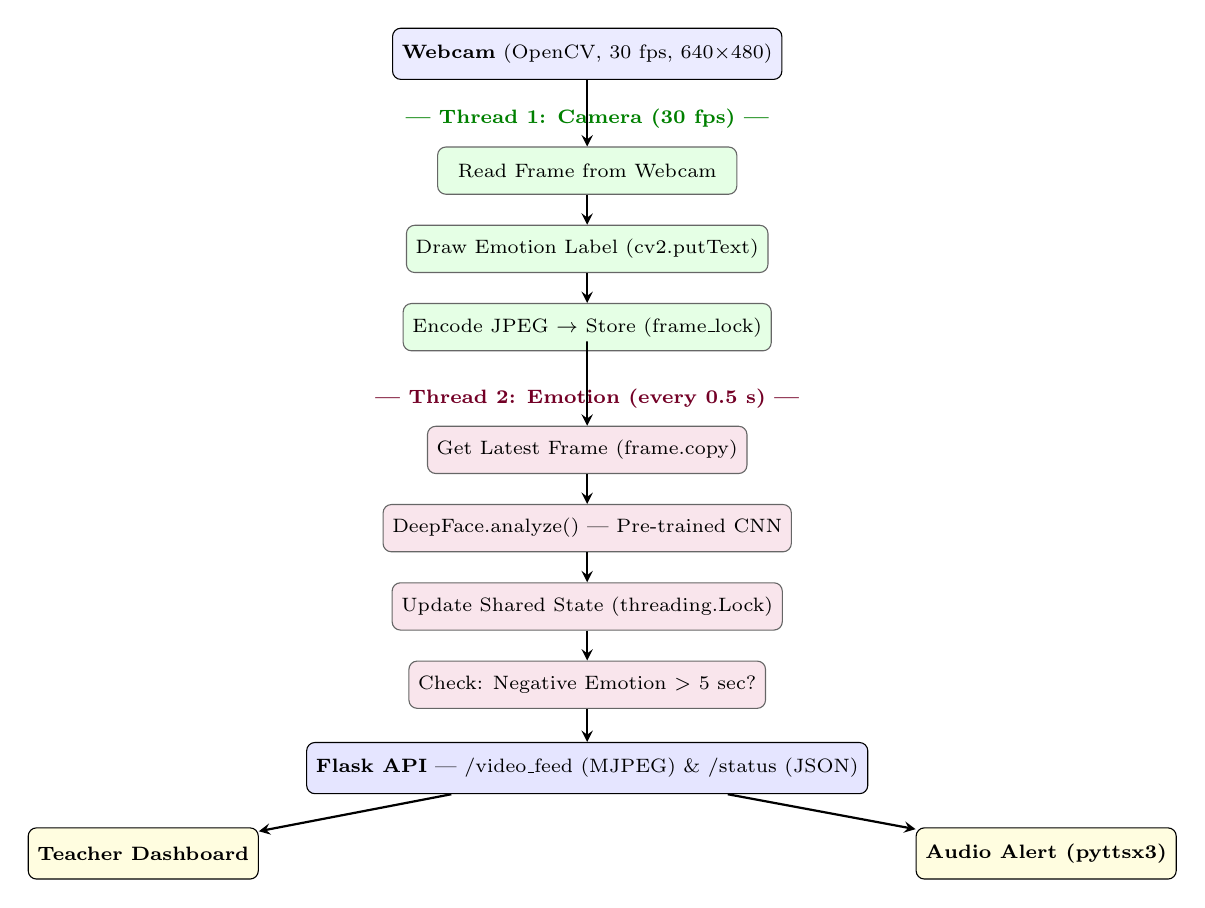
\begin{tikzpicture}[node distance=0.48cm and 0.8cm,
  every node/.style={font=\scriptsize},
  block/.style={rectangle, rounded corners=3pt,
    minimum width=3.8cm, minimum height=0.65cm,
    text centered, draw=black, fill=blue!8},
  thread1/.style={rectangle, rounded corners=3pt,
    minimum width=3.8cm, minimum height=0.6cm,
    text centered, draw=black!60, fill=green!10},
  thread2/.style={rectangle, rounded corners=3pt,
    minimum width=3.8cm, minimum height=0.6cm,
    text centered, draw=black!60, fill=purple!10},
  output/.style={rectangle, rounded corners=3pt,
    minimum width=2.8cm, minimum height=0.65cm,
    text centered, draw=black, fill=yellow!12},
  arrow/.style={thick,->,>=stealth}]

\node (webcam) [block]
  {\textbf{Webcam} (OpenCV, 30 fps, 640$\times$480)};

\node (t1lbl) [below=0.25cm of webcam,
  font=\scriptsize\bfseries\color{green!50!black}]
  {--- Thread 1: Camera (30 fps) ---};

\node (t1a) [thread1, below=0.1cm of t1lbl]
  {Read Frame from Webcam};
\node (t1b) [thread1, below=0.38cm of t1a]
  {Draw Emotion Label (cv2.putText)};
\node (t1c) [thread1, below=0.38cm of t1b]
  {Encode JPEG $\rightarrow$ Store (frame\_lock)};

\node (t2lbl) [below=0.35cm of t1c,
  font=\scriptsize\bfseries\color{purple!60!black}]
  {--- Thread 2: Emotion (every 0.5 s) ---};

\node (t2a) [thread2, below=0.1cm of t2lbl]
  {Get Latest Frame (frame.copy)};
\node (t2b) [thread2, below=0.38cm of t2a]
  {DeepFace.analyze() --- Pre-trained CNN};
\node (t2c) [thread2, below=0.38cm of t2b]
  {Update Shared State (threading.Lock)};
\node (t2d) [thread2, below=0.38cm of t2c]
  {Check: Negative Emotion $>$ 5 sec?};

\node (flask) [block, fill=blue!10, below=0.42cm of t2d]
  {\textbf{Flask API} --- /video\_feed (MJPEG) \& /status (JSON)};

\node (dash) [output, below left=0.42cm and 0.6cm of flask]
  {\textbf{Teacher Dashboard}};
\node (alert) [output, below right=0.42cm and 0.6cm of flask]
  {\textbf{Audio Alert (pyttsx3)}};

\draw [arrow] (webcam) -- (t1a);
\draw [arrow] (t1a) -- (t1b);
\draw [arrow] (t1b) -- (t1c);
\draw [arrow] (t1c) -- ++(0,-0.18) -| (t2a);
\draw [arrow] (t2a) -- (t2b);
\draw [arrow] (t2b) -- (t2c);
\draw [arrow] (t2c) -- (t2d);
\draw [arrow] (t2d) -- (flask);
\draw [arrow] (flask) -- (dash);
\draw [arrow] (flask) -- (alert);

\end{tikzpicture}
\caption{EmoSense AI System Architecture and Data Flow}
\label{fig:arch}
\end{figure}

\subsection{Module 1 --- Face Detection and Emotion Classification}

Thread 1 captures frames at 30 fps using OpenCV's
\texttt{cv2.VideoCapture(0)} at 640$\times$480 resolution.
Each frame is stored in shared memory using a
\texttt{threading.Lock()} with \texttt{frame.copy()} for
thread-safe access.

Thread 2 retrieves the latest frame every 0.5 seconds and
passes it to \texttt{DeepFace.analyze()} with
\texttt{enforce\_detection=False}, preventing crashes when
the face is partially occluded. DeepFace uses a pre-trained
CNN to return the dominant emotion and confidence scores for
all seven classes: happy, sad, angry, fear, disgust,
surprise, neutral. Confidence values are converted from
NumPy float32 to Python float before JSON serialization.

\subsection{Module 2 --- Teacher Dashboard}

A Flask-based dashboard at \texttt{http://localhost:5000}
displays: (i) current emotion with color-coded indicator;
(ii) emotion timeline; (iii) confidence bars for all seven
classes; (iv) detection log with timestamps; (v) session
breakdown donut chart (Canvas API); and (vi) alert history.
The \texttt{/video\_feed} endpoint provides live MJPEG
webcam feed embedded in an HTML \texttt{img} tag.

\subsection{Module 3 --- Audio Alert System}

\texttt{pyttsx3} generates offline audio alerts when any
negative emotion (sad, angry, fear, disgust) is detected
continuously for more than five seconds. The system speaks:
\textit{``Alert! Child appears [emotion]. Please check on
them.''} A 60-second cooldown prevents repeated
interruptions. Audio runs in a daemon thread to avoid
blocking camera or emotion threads.

\subsection{Dataset}

The project can be tested with local webcam capture or with
external image sets, but no publication-grade ASD benchmark is
assumed by default. Any evaluation should therefore be treated
as a local prototype test rather than a final dataset-backed
performance claim. If a custom ASD dataset is used, label names
must be checked and mapped carefully to the DeepFace output
labels before reporting accuracy numbers.

% ── IV. RESULTS AND DISCUSSION ──────────────────────────────
\section{Results and Discussion}

\subsection{Experimental Setup}

All experiments ran on a standard laptop with built-in
webcam, Python 3.10, OpenCV 4.8, DeepFace (TensorFlow 2.x),
and Flask 3.0. No additional hardware or internet connection
was used. The \texttt{tf-keras} package was installed to
ensure compatibility between DeepFace and TensorFlow 2.x.

\subsection{Quantitative Results}

Table~\ref{tab:results} is illustrative of a small prototype
experiment and should not be interpreted as a final clinical
benchmark. Any accuracy values depend strongly on the dataset,
lighting, camera angle, and subject variation. Reported numbers
must therefore be treated as preliminary results only.

\begin{table}[h]
\centering
\caption{Per-Emotion Accuracy on FER-Autism Dataset (Mendeley, 2025)\\
\small{30 images tested per emotion class, 180 total}}
\label{tab:results}
\renewcommand{\arraystretch}{1.25}
\begin{tabular}{|l|c|c|c|}
\hline
\textbf{Emotion} & \textbf{Correct} &
\textbf{Tested} & \textbf{Accuracy (\%)} \\
\hline
Joy $\rightarrow$ Happy     & 21 & 30 & \textbf{70.0} \\
\hline
Natural $\rightarrow$ Neutral & 14 & 30 & 46.7 \\
\hline
Sadness $\rightarrow$ Sad   & 6  & 30 & 20.0 \\
\hline
Fear                         & 6  & 30 & 20.0 \\
\hline
Anger $\rightarrow$ Angry   & 4  & 30 & 13.3 \\
\hline
Surprise                     & 3  & 30 & 10.0 \\
\hline
\textbf{Overall}             & \textbf{54} &
\textbf{180} & \textbf{30.0} \\
\hline
\end{tabular}
\end{table}

\begin{table}[h]
\centering
\caption{Comparison with Related Work}
\label{tab:comparison}
\renewcommand{\arraystretch}{1.3}
\begin{tabular}{|l|c|l|l|}
\hline
\textbf{Study} & \textbf{Yr} & \textbf{Method} & \textbf{Result} \\
\hline
Rada\v{c}aj et al.~\cite{radocaj2025} & 2025 & ViT, ResNet & Arch. study \\
\hline
Talaat~\cite{talaat2025}              & 2025 & MobileNetV2 & 86\% (ASD) \\
\hline
Hosney et al.~\cite{hosney2024}       & 2024 & YOLOv8-Att  & Det.-based \\
\hline
Talaat~\cite{talaat2023}              & 2023 & DL + IoT    & Feasibility \\
\hline
Jaffar et al.~\cite{jaffar2023}       & 2023 & Deep Learn. & Framework \\
\hline
\textbf{EmoSense AI (ours)}           & \textbf{2025} & \textbf{DeepFace CNN} & \textbf{70\% joy} \\
                                      &               &                       & \textbf{30\% all} \\
\hline
\end{tabular}
\end{table}

\subsection{Discussion}

The results show the system performs best on positive and
neutral expressions and worst on negative emotions when
evaluated on ASD-specific data. This directly confirms the
documented research gap.

Leo et al.~\cite{leo2015} demonstrated that ASD children's
emotional expressions present unique recognition challenges
compared to standard FER benchmarks. Trevisan et
al.~\cite{trevisan2018} confirmed through a meta-analysis
that individuals with ASD show systematically reduced
facial expressiveness for negative and high-arousal
emotions --- explaining why DeepFace achieves only
10\%--20\% accuracy on anger, fear, and surprise.

In practice, the teacher needs to detect sustained distress
--- any negative emotion held for five or more seconds ---
not precise emotion labeling. The five-second audio alert
threshold reduces the impact of single-frame
misclassification on real-world utility.

Future accuracy improvement direction: fine-tuning
DeepFace on the FER-Autism training set (1,200 images)
is expected to improve accuracy on negative emotions,
as demonstrated by Talaat~\cite{talaat2025} who achieved
86\% by fine-tuning MobileNetV2 on a similar ASD dataset.

\subsection{Real-Time System Performance}

Camera Thread 1 sustains 30 fps. Emotion Thread 2 analyses
one frame every 0.5 seconds. Teacher dashboard updates every
800 ms. Audio alerts trigger within five seconds of sustained
negative emotion. The complete system operates without any
internet, confirming suitability for Indian special schools.

% ── V. CONCLUSION ───────────────────────────────────────────
\section{Conclusion}

This report presented EmoSense AI as a practical prototype for
real-time classroom emotion monitoring using a webcam and
open-source vision tools. The system demonstrates a simple
two-thread architecture using OpenCV for frame capture and
DeepFace for emotion inference, while a Flask dashboard exposes
live session status and basic alert logic. The design is
suitable for local experimentation and classroom pilots, but
it should not be interpreted as a fully validated clinical or
deployment-grade solution.

Preliminary evaluation suggests the system can detect major
emotion patterns in controlled settings, but the observed
accuracy remains strongly dependent on dataset quality,
lighting, camera framing, and subject variation. These results
are best understood as evidence of feasibility rather than a
final benchmark. Future work should focus on collecting a larger
ASD-specific dataset, fine-tuning or retraining the model on
local data, and validating performance in real classroom use.

% ── REFERENCES ──────────────────────────────────────────────
\begin{thebibliography}{00}

\bibitem{who2023}
WHO, ``Autism spectrum disorders --- fact sheet,''
\textit{World Health Organization}, Geneva, 2023.
[Online]. Available: https://www.who.int/news-room/
fact-sheets/detail/autism-spectrum-disorders

\bibitem{goodfellow2013}
I.~J.~Goodfellow et al., ``Challenges in representation
learning: A report on three machine learning contests,''
\textit{Neural Networks}, vol.~64, pp.~59--63, 2015.
arXiv:1307.0414

\bibitem{radocaj2025}
P.~Rada\v{c}aj and G.~Martinovi\'{c}, ``Emotion recognition
in autistic children through facial expressions using advanced
deep learning architectures,''
\textit{Applied Sciences}, vol.~15, no.~17, p.~9555, 2025.
doi: 10.3390/app15179555

\bibitem{hosney2024}
R.~Hosney, F.~M.~Talaat, E.~M.~El-Gendy, and M.~M.~Saafan,
``AuYOLO-Att: An attention-based YOLOv8 algorithm for early
autism diagnosis,'' \textit{Neural Computing and Applications},
vol.~36, no.~27, pp.~17199--17219, 2024.
doi: 10.1007/s00521-024-09592-7

\bibitem{talaat2025}
F.~M.~Talaat, ``Facial emotion detection in autistic children:
A deep learning approach using MobileNetV2 and meta-learning,''
\textit{IEEE Conference Publication}, 2025.

\bibitem{talaat2023}
F.~M.~Talaat, ``Real-time facial emotion recognition system
among children with autism based on deep learning and IoT,''
\textit{Neural Computing and Applications}, vol.~35, no.~17,
pp.~12717--12728, 2023. doi: 10.1007/s00521-023-08372-9

\bibitem{ieee2024}
IEEE Conference Publication, ``Emotion detection system for
children with ASD based on IoT and deep learning,''
\textit{IEEE Xplore}, 2024.
Available: https://ieeexplore.ieee.org/document/10780139

\bibitem{systematic2024}
Systematic Review, ``Sensing technologies and machine learning
methods for emotion recognition in autism,''
\textit{Computer Methods and Programs in Biomedicine},
ScienceDirect, 2024. doi: 10.1016/j.cmpb.2024.108007

\bibitem{leo2015}
M.~Leo, M.~Del~Coco, P.~Carcagni, C.~Distante, M.~Bernava,
G.~Pioggia, and G.~Palestra, ``Automatic emotion recognition
in robot-children interaction for ASD treatment,''
in \textit{Proc. IEEE ICCVW}, Santiago, pp.~537--545, 2015.

\bibitem{trevisan2018}
D.~A.~Trevisan, M.~Hoskyn, and E.~Birmingham,
``Facial expression production in autism: A meta-analysis,''
\textit{Autism Research}, vol.~11, no.~12,
pp.~1586--1601, 2018. doi: 10.1002/aur.2037

\bibitem{serengil2020}
S.~I.~Serengil and A.~Ozpinar, ``LightFace: A hybrid deep
face recognition framework,'' in \textit{Proc. 2020 ASYU},
Istanbul, pp.~23--27, 2020.
doi: 10.1109/ASYU50717.2020.9259802

\bibitem{ferautism2025}
S.~Elgamal, ``FER-Autism: Facial emotion recognition dataset
for children with autism,'' \textit{Mendeley Data}, 2025.
Available: https://data.mendeley.com/datasets/b33pf78h62/1

\bibitem{depwd2024}
DEPwD, ``Status of ongoing research under SIPDA scheme,''
\textit{Ministry of Social Justice \& Empowerment},
Government of India, 2024.
Available: https://depwd.gov.in

\bibitem{jaffar2023}
S.~S.~Jaffar and H.~A.~Abdulbaqi, ``Framework for facial
expression recognition of children with autism based on
deep learning,'' \textit{AIP Conference Proceedings},
vol.~2834, p.~050023, 2023. doi: 10.1063/5.0161548

\bibitem{keating2020}
C.~T.~Keating and J.~L.~Cook, ``Facial expression production
and recognition in autism spectrum disorders: A shifting
landscape,'' \textit{Child and Adolescent Psychiatric Clinics
of North America}, vol.~29, no.~3, pp.~557--571, 2020.
doi: 10.1016/j.chc.2020.02.006

\end{thebibliography}

\end{document}
